%! TEX root = 'main.tex'

\section{Evaluation}
\label{sec:evaluation}

In this section, we evaluates performance overhead and how it protets  operating system from real-world vulnerabilities.

\subsection{Performance}
In this section, we focus on performance evaluation. 
As formerly mentioned, this project has two major parts, the hypervisor, and the exception handler. To accurately presents the performance impact that introduced by this mitigation. We conduct the tests in three parts.

Firstly, the hypervisor plays an essential part in this project. Without it, the SMAP exception would happen within any context, even in the path of handling the previous case. Nowadays, a hypervisor is part of the infrastructure of cloud computing. Even the Windows 10 operating system brings its native hypervisor to achieve security goals.  Therefore, in those scenarios,  the performance overhead introduced by the hypervisor pre-existed. 

In this part, we use the well-known benchmark SPEC 2006. We understand that this benchmark is for instruction evaluation, specifically for microarchitectural aspects, such as instruction execution, branch prediction accuracy, cache policies. We choose several programs from the set, all without GUI and computational intensive comparing to the fewer system calls. Therefore the performance overhead incurred is mainly from the hypervisor.

We compare our hypervisor with vanilla OS and the native Windows 10 hypervisor used for code integrity purposes. We are not trying to compete with HVCI (Windows 10 native hypervisor) because the two hypervisors serve different objectives. But to show at what level, the end-user may accept a hypervisor by default.


All tests run on the PC: Intel Core I5-6400 (6 GEN CPU Skylake), ASUS H110M-C mother board(Intel H110 Chipset, Realtek RTL8111H Network Controller), 8GB RAM and 500GB hard disk.


\begin{figure}[th]
  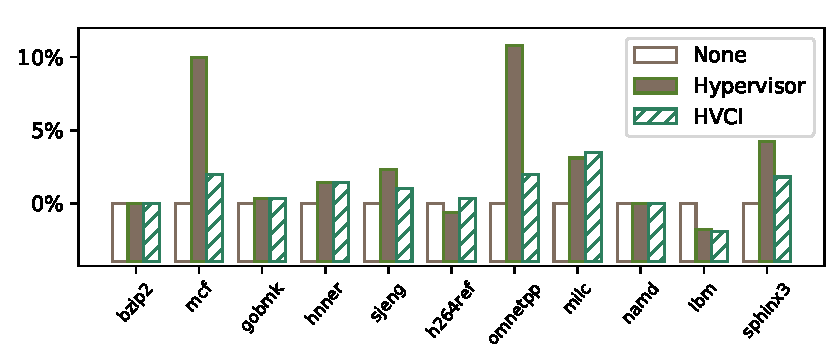
\includegraphics[width=0.47\textwidth]{figures/benchmark3}
  \centering
  \caption{Performance overhead on the SPEC benchmarks incurred by the run-time load hypervisor. HVCI represent the Windows 10 native hypervisor for Hypervisor-Protected Code Integrity. All overheads are normalized to the unprotected system running benchmark.}
  \label{fig:benchmark}
\end{figure}

As shown in~\autoref{fig:benchmark}, the performance overhead of hypervisor alone is acceptable, on average, 3.25\%. HVCI yields a modest performance overhead of 0.81\%.

Our hypervisor is slower, particularly in two benchmark programs. Learning more about computer architecture and virtualization techniques, we wish to improve our hypervisor to achieve the same performance.

We chose several non-trivial applications to demonstrate the performance overhead introduced by our mitigation. Systematic mitigation is difficult, especially for an operating system as complicated as Windows. Those ones run long enough to make the tests possible.

\begin{figure}[th]
  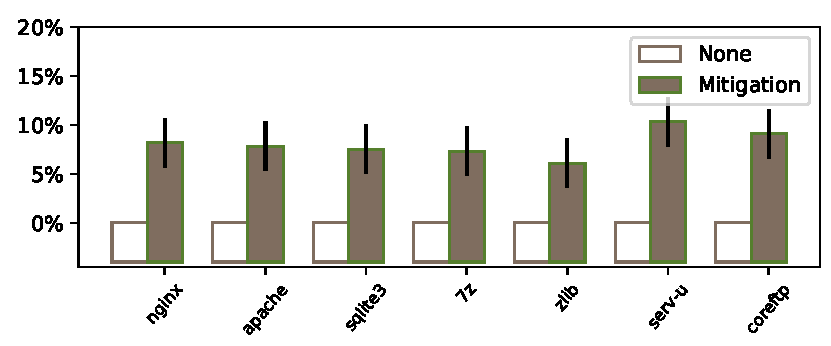
\includegraphics[width=0.47\textwidth]{figures/performance4}
  \centering
  \caption{Performance overhead in non-trivial applications. Overhead mostly being introduced on system calls that need to fetch user-mode parameters}
  \label{fig:performance}
\end{figure}

~\autoref{fig:performance} shows the performance overhead of our mitigation in several non-trivial application. Some of those applications potentially could be the trampoline service of kernel TOCTOU attacks.
For web server software such as Nginx. We test its performance by counting the accumulated response time for 10000 web requests. For compression software such as zlib, we test it with compressing large files. For sqlite3, we use speedtest1.c which is a common performance testing program.

The result shows that the performance overhead is acceptable. Because only the system calls that have user-mode buffer as their parameters will trigger SMAP exceptions. 



Based on our investigation through reverse-engineering and monitoring, we find that the Windows kernel's graphical module, namely, win32k.sys, has the most TOCTOU issue. Due to the nature of how the GUI subsystem drawing screen, the number of win32k system calls is tremendous, even for a simple program such as Windows notepad. The GUI system calls frequently reference user-mode variables. Some of the cases fall into the kernel TOCTOU category; the others are benign. We believe that the situation will be eased with the improvement of the new Windows kernel. Because of the formerly mentioned two causes, our mitigation incurs an unneglectable performance overhead when applied to GUI programs. If the GUI window minimized, the screen drawing related system calls are stopped, but the rest is still in service. This is the case for most server services.


To measure the number of system calls, we drag the GUI program's window around to let the system redraw the screen. For the server programs, the results depend on the requests it served. We send a URL request for the default page every second. 

We take 500 system calls as the standard to measure the following: how many pages touched and protected, how much time does the program took, and how many double fetches happened.

\begin{center}
\begin{table}
	\small
	%\renewcommand{\arraystretch}{1.3}
	\caption{System call count and user-pages accessed for GUI \& non-GUI programs }
	\label{table:pages}
	\centering
%	\begin{tabular}{ l|p{0.04\textwidth}|p{0.108\textwidth}|l|p{0.045\textwidth}|p{0.045\textwidth} } 
%	\begin{tabular}{ c@{}|@{}c@{}|@{}c@{}|@{}c@{}|@{}c@{}|@{}c }   
	\begin{tabular}{@{}>{\centering\arraybackslash}m{1.35cm}@{}|
			@{}>{\centering\arraybackslash}m{1.10cm}@{}|
			@{}>{\centering\arraybackslash}m{2.20cm}@{}|
			c|
			@{}>{\centering\arraybackslash}m{1.10cm}@{}|
			@{}>{\centering\arraybackslash}m{0.92cm}@{} } 
		\hline
		Programs & System Calls & Protected Pages(r, w) & \textbf{avg.} & Double Fetch & Time (ms)\\ 
		\hline
		nginx & 500 & 711(711, \textbf{0}) & 1.42 & \textbf{223} &12312\\ 
		apache & 500 & 689(689, \textbf{0})  & 1.38 & \textbf{205} &11339\\ 
		notepad & 500 & 1434(1102, 241) & 2.87 & \textbf{1373} & 1859 \\ 
		freecell & 500 & 1352(1165, 187) & 2.70 & \textbf{1266} & 1500 \\ 
		\hline
	\end{tabular}
\end{table}
\end{center}

%\begin{center}
%\begin{table}[ht]
%	\small
%	%\renewcommand{\arraystretch}{1.3}
%	\caption{System call count and user-pages accessed for GUI \& non-GUI programs }
%	\label{table:pages}
%	\centering
%	\begin{tabular}{>{\centering\arraybackslash}m{1.35cm}|
%		        >{\centering\arraybackslash}m{1.1cm}|c|c|
%		 	>{\centering\arraybackslash}m{1.1cm}|
%			>{\centering\arraybackslash}m{0.92cm} } 
%		\hline
%		Programs & System Calls & Pages & \textbf{avg.} & Double Fetch & Time (ms)\\ 
%		\hline
%		nginx & 500 & 711 & 1.42 & \textbf{223} &12312\\ 
%		apache & 500 & 689 & 1.38 & \textbf{205} &11339\\ 
%		notepad & 500 & 1434 & 2.87 & \textbf{1373} & 1859 \\ 
%		freecell & 500 & 1352 & 2.70 & \textbf{1266} & 1500 \\ 
%		\hline
%	\end{tabular}
%\end{table}
%\end{center}

As shown in~\autoref{table:pages}, even without any explicit interactive operation, refreshing the GUI takes tremendous system calls. Services such as Nginx only have few system calls when idle. On average,  the win32k system call accesses more user pages than the kennel system call does. One reason is that other than "capturing" the user-supplied parameter at the beginning of a system call, win32k read/writes user variables even during the system call. 



% use this with the previous table with Protected Page(r,w)
Among those pages, we also record the access type, either read or write. It is the type of which the kernel first accesses a user page, triggering a SMAP exception. We notice that the number of write-access pages is zero for non-GUI programs. It appears that the kernel does not directly write user pages, which is false. The reasons are the following.  The operating system provides the three methods for accessing data buffers: Buffered I/O, Direct I/O, and Neither Buffered Nor Direct I/O.

Buffered I/O and Neither I/O can copy or write to a user buffer, but Direct I/O is the most common way to transfer amounts of data. The operating system locks the application's buffer in memory. It then
creates a memory descriptor list (MDL) that identifies the locked memory pages and passes the MDL to the driver stack. Drivers access the locked pages through the MDL.

However, the system still needs to fill in some parameters directly, such as a word-size handle from the system call ZwCreateFile. As described earlier, the kernel calls ProbeForWrite inside a try-catch block.

For example, the pseudo-code for validating the filehandle parameter is similar to the following.


\begin{lstlisting}[style=code, caption={Pseudo-code of kernel validating a user-supplied variable. } \label{lst:probeforwrite}, captionpos=b]
try {
	...
	*((volatile HANDLE *)Address) = *Address;

} except(EXCEPTION_EXECUTE_HANDLER) {

	// Error handling
	return GetExceptionCode();
}
\end{lstlisting}

We can see that the assembly code generated always reads the variable before writing it. This coding style is another cause for the zero write access. 


% for later reference
%Buffered I/O
%The operating system creates a nonpaged system buffer, equal in size to the application's buffer. The I/O manager copies user data into the system buffer for write operations before calling the driver stack. For read operations, the I/O manager copies data from the system buffer into the application's buffer after the driver stack completes the requested operation.
%
%Direct I/O
%The operating system locks the application's buffer in memory. It then creates a memory descriptor list (MDL) that identifies the locked memory pages and passes the MDL to the driver stack. Drivers access the locked pages through the MDL.
%
%Neither Buffered Nor Direct I/O
%The operating system passes the application buffer's virtual starting address and size to the driver stack. The buffer is only accessible from drivers that execute in the application's thread context.
%



The column "Double Fetch" shows the user-addresses that are read over twice during a system call. We trace this information with an alternative project. It shows the win32k has more cases than the kernel. These potentially are double-fetch candidates. There exist duplicate records, and a significant proportion of the target addresses are within Process Environment Block(PEB) or Thread Environment Block(TEB) pages.  The selected logs we give below are during various system calls.  Every two rows show that a potential subsequent instruction revisits the same user address shortly after. From the Cr3 and Teb values, it is the same thread of the same process. We observe that some instances fall under this category are direct access, even without a try-catch block. This finding also proves the necessity of such run-time mitigation for kernel TOCTOU vulnerability.


%\begin{center}
%\begin{table}
%	\renewcommand{\arraystretch}{1.3}
%	\caption{Some of the double-fetch results. }
%	\label{table:doubleread}
%	\centering
%	\begin{tabular}{ l } 
%		\hline
%		Results: \\
%		\hline
%		CR3 0x6d40320 EIP 0xbf812de4 Addr 0x4808c4 TEB 0x7ffdd000 \\
%		CR3 0x6d40320 EIP 0xbf812e4b Addr 0x4808c4 TEB 0x7ffdd000 \\
%		\hline
%		CR3 0x6d40320 EIP 0xbf812dea Addr 0x4808c8 TEB 0x7ffdd000 \\
%		CR3 0x6d40320 EIP 0xbf812e55 Addr 0x4808c8 TEB 0x7ffdd000 \\
%		\hline
%		CR3 0x6d40320 EIP 0xbf812daf Addr 0x480750 TEB 0x7ffdd000 \\
%		CR3 0x6d40320 EIP 0xbf812e21 Addr 0x480750 TEB 0x7ffdd000 \\
%		\hline
%		CR3 0x6d40320 EIP 0xbf80c04d Addr 0x7ffdd206 TEB 0x7ffdd000 \\
%		CR3 0x6d40320 EIP 0xbf812ebe Addr 0x7ffdd206 TEB 0x7ffdd000 \\
%		\hline
%	\end{tabular}
%\end{table}
%\end{center}


\begin{center}
	\begin{table}[ht]
		\small
		\renewcommand{\arraystretch}{1.2}
		\caption{Some of the double-fetch results. }
		\label{table:doubleread}
		\centering
		\begin{tabular}{ l l l l }
			\hline
			Cr3 & Eip & Addr. & Teb \\
			\hline
			0x6d40320 & 0xbf812de4 & \textbf{0x4808c4} & 0x7ffdd000 \\
			0x6d40320 & 0xbf812e4b & \textbf{0x4808c4} & 0x7ffdd000 \\
			\hline
			0x6d40320 & 0xbf812dea & \textbf{0x4808c8} & 0x7ffdd000 \\
			0x6d40320 & 0xbf812e55 & \textbf{0x4808c8} & 0x7ffdd000 \\
			\hline
			0x6d40320 & 0xbf812daf & \textbf{0x480750} & 0x7ffdd000 \\
			0x6d40320 & 0xbf812e21 & \textbf{0x480750} & 0x7ffdd000 \\
			\hline
			0x6d40320 & 0xbf80c04d & 0x7ffdd206 & 0x7ffdd000 \\
			0x6d40320 & 0xbf812ebe & 0x7ffdd206 & 0x7ffdd000 \\
			\hline
		\end{tabular}
	\end{table}
\end{center}



%Part of the overhead is introduced due to the overall intercepting of page fault exceptions of the system. The page fault handler is called in high frequency. Our page fault hook currently is installed directly in the IDT table of each processor. Hence every page fault exception goes through our handler. Even though, in the very begining, we pass through exceptions that doesn't belong to the target process, still extra instructions are executed for each exception.

%Although we use virtualization techniques, but the hypervisor we use is a very simple one. Unlike commercial virtualization solutions such as VMWare, Xen and Qemu+Kvm, ours doesn't emulate any hardware devices nor intercept further page mapping translate that between host and guest. Only several types of VM-Exit is inevitable such as control register accessing which we do need to handle it too.

Considering the kernel is fully aware of the untrustworthy user-supplied parameters, we believe it is practical to eliminate the SMAP exceptions during parameter validating. It will promote the performance of mitigation. As was done with the Linux kernel, the SMAP feature is temporarily disabled during copy\_from\_user() and copy\_to\_user(), the gateways. In Windows kernel, ProbeForRead() and ProbeForWrite() are the equivalent of that. However, such "Probe" has many variants. For example, ProbeAndWriteHandle(), ProbeForWriteIoStatus(). Some of them are macros instead of functions, making it difficult to change all of them without recompiling the kernel. On the contrary, the code piece that uses user variable is spreading across the module. The repairing process will take great effort. 

\subsection{Case Study}

CVE-2008-2252 is a typical TOCTOU vulnerability which is analyzed as a example in many previous researches. To evaluate the effectiveness of our mitigation, We tested it on a desktop with Windows XP installed. It's troublesome to install an old Windows operating system on a modern PC, particularly, because modern chipset which integrated hard disk controller no longer support IDE mode. Hence we need ASUS AHCI driver for Windows XP, tool that can make a USB stick bootable and tool that virtualize a floppy drive~\cite{installxpskylake} for providing AHCI driver during the installation.
We write a proof-of-concept(POC) program to test our mitigation against CVE-2008-2252. It triggers the TOCTOU vulnerability to introduce a memory buffer overflow. 

%We test it on the Windows XP sp3 system with the vulnerable win32k.sys file whose version is 5.1.2600.5512. Because SMAP only available at Intel 5th generation CPU (architecture code name Broadwell). Hard-disk controller which integrated in the CPU corresponded chipset doesn't support ATA mode anymore, and Windows XP system doesn't support AHCI mode, so it's difficult to install it on a modern PC. Our testing environment is established using a virtual machine. Particularly, VMWare Workstation 14 Player, emulated "Intel Core i5-6200U CPU (2 cores) with 1GB of RAM", option "Virtualize Intel VT-x/EPT or AMD-v/RVI" also enabled.

The attacking program has two threads. The main thread first allocate a page at virtual address 0, which later used as the parameter to be sent into the vulnerable syscall. The reason to choose page zero is to bypass the parameter check in syscall NtUserMessageCall. Next, right after creating another thread, it keeps calling the vulnerable function SendMessage (WM\_COPYDATA) with the malicious parameters in a loop, which eventually calls the vulnerable win32k function xxxInterSendMsgEx. The created thread then keep modifying the parameter at page zero, also in a loop, simultaneously.

\begin{figure}[th]
  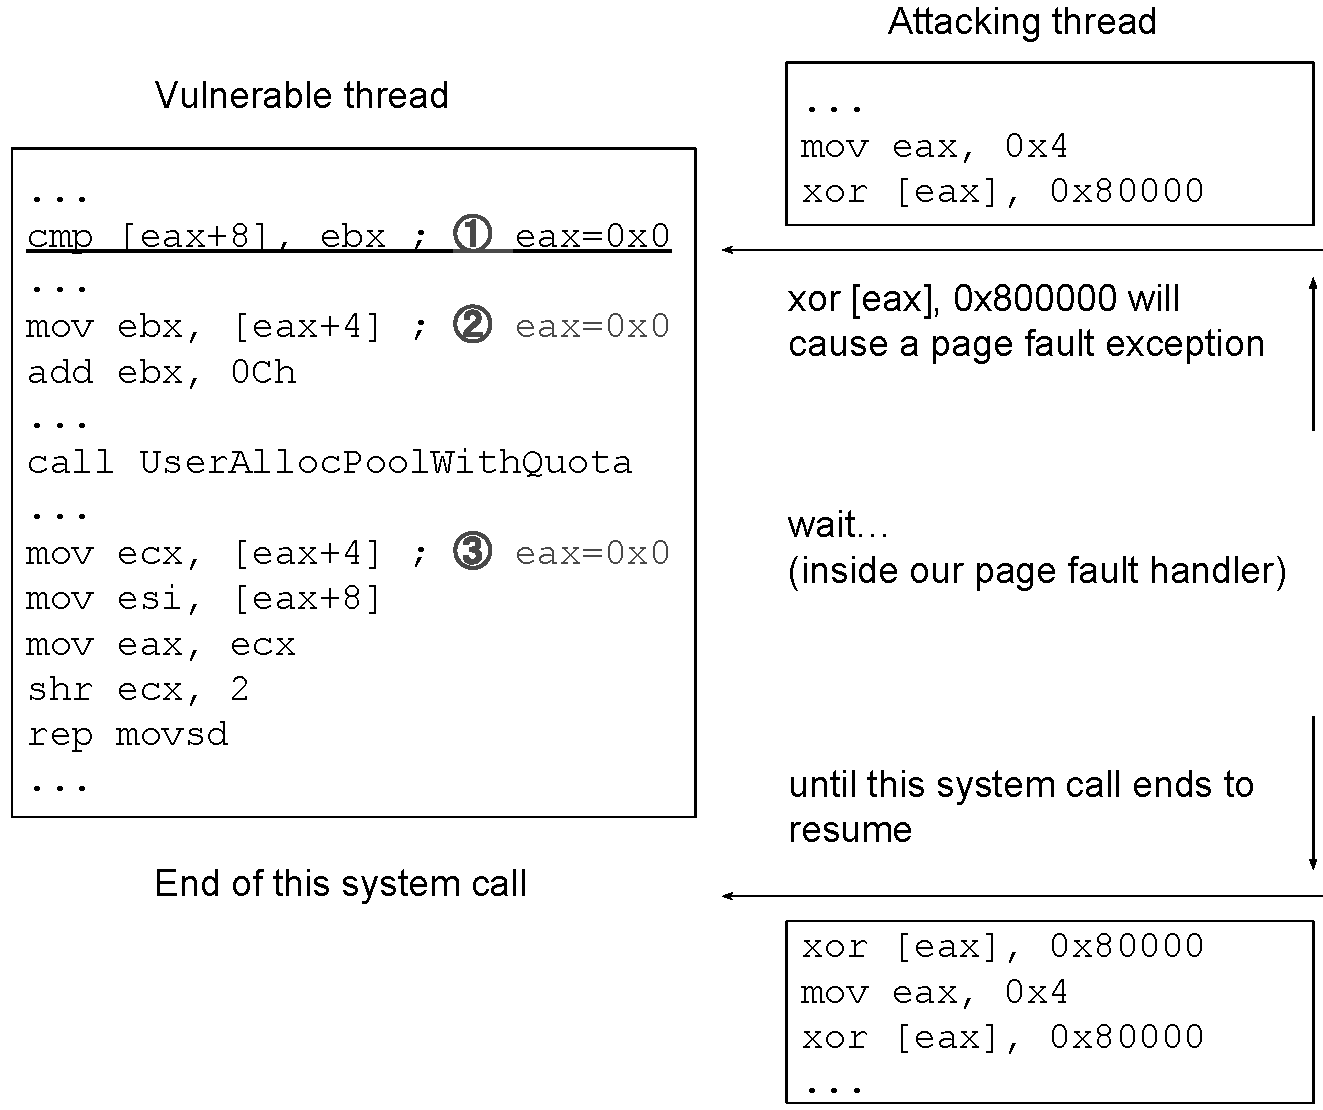
\includegraphics[width=0.47\textwidth]{figures/ms08061case}
  \centering
  \caption{The user page will be protected right at the moment it's been referenced.}
  \label{fig:ms08061case}
\end{figure}

In the attack, as shown in ~\autoref{fig:ms08061case}, the \textcircled{2} and \textcircled{3} are the places where vulnerable user-mode variable pcbData are referenced, it's address is 0x4. But the first time the zero page get accessed is \textcircled{1} where several instruction ahead of \textcircled{2}, it triggers an page fault exception (cased by SMAP). Therefore this page will be marked as a kernel page by our page fault handler. From this moment until the end of the current system call, this page will be protected from modifying by either as a kernel page or a user page with read-only permit. If the attacking thread try to modified it, another page fault exception  will be raised because of access violation. Then the attacking thread will be held for 30 milliseconds before it try to re-execute the faulting instruction again, for as many as 10 times. If not possible, the attacking thread will be terminated. We can see that during the protection, memory reads at \textcircled{2} and \textcircled{3} are kept consistent.


CVE-2013-1254 is another typical TOCTOU vulnerability that found in Windows win32k module~\cite{jurczyk2013identifying}. It effects both Windows XP and Windows 7. 

%A series of same kind of vulnerability found in 26 functions of module win32k.

\begin{lstlisting}[style=code] 
.text:BF8A993F   mov   eax, _W32UserProbeAddr
                       .
                       .
.text:BF8A9973   @cmp   [ecx+8], eax@    
.text:BF8A9976   jnb   short loc_BF8A997B
.text:BF8A9978   @mov   eax, [ecx+8]@    
.text:BF8A997B
.text:BF8A997B loc_BF8A997B:                           
.text:BF8A997B   mov   ecx, [eax]
.text:BF8A997D   mov   eax, [eax+4]
\end{lstlisting}
%\captionof{lstlisting}{Flawed code in win32k.sys function SfnINOUTSTYLECHANGE()}

The flawed function first fetch a value from "ecx+8" and compare it with \_W32UserProbeAddress which is a value that indicates the highest possible address for user-mode variables. It confirms that the variable is actually reside in user space. Next, it fetches the value again and assign it to eax. This is where the double fetch happens. The attacker can change the value between those two fetches, letting it bypass the verification,  then assign it a kernel space address.

So when "ecx+8" is referenced the first time, the corresponding page will trigger a SMAP exception, then this page will be protected until the current system call ends. Other threads write to it will also trigger page fault exceptions, as explained in the previous case, out page fault handler will handle those to keep the data consistent. 


